% !Mode:: "TeX:UTF-8"

\documentclass[12pt,oneside]{book}

\newlength{\textpt}
\setlength{\textpt}{12pt}
    
%========基本必备的宏包========%
\RequirePackage{calc,float,moresize}
%\RequirePackage[onehalfspacing]{setspace}
\linespread{1.5}
%1.3 onehalfspacing
%1.6 doublespacing

%===========加入目录 某章或某节=====%
\makeatletter

\newcommand{\addchtoc}[1]{
        \cleardoublepage
        \phantomsection
        \addcontentsline{toc}{chapter}{#1}}

\newcommand{\addsectoc}[1]{
        \phantomsection
        \addcontentsline{toc}{section}{#1}}

%===========全文基本格式==========%
\setlength{\parskip}{1.6ex plus 0.2ex minus 0.2ex}   %段落間距
\setlength{\parindent}{\textpt * \real{2}}
\RequirePackage{indentfirst} 

%=========页面设置=========%
\RequirePackage[a4paper, %a4paper size 297:210 mm
  bindingoffset=0mm,%裝訂線
  top=35mm,  %上邊距 包括頁眉
  bottom=30mm,%下邊距 包括頁腳
  inner=30mm,  %左邊距or inner
  outer=30mm,  %右邊距or  outer
  headheight=10mm,%頁眉
  headsep=15mm,%
  footskip=15mm,%
  marginparsep=0pt, %旁註與正文間距
  marginparwidth=0em,includemp=false% 旁註寬度計入width%旁註寬度
  ]{geometry}

%color
\RequirePackage[table,svgnames]{xcolor}

%================字體================%
%设置数学字体
\RequirePackage{amssymb,amsmath}
\RequirePackage{stmaryrd}
\everymath{\displaystyle}

\RequirePackage{fontspec}
%設置英文字體
\setmainfont[Mapping=tex-text]{DejaVu Serif}
\setsansfont[Mapping=tex-text]{DejaVu Sans}
\setmonofont[Mapping=tex-text]{DejaVu Sans Mono}


%中文環境
\RequirePackage[]{xeCJK}
\xeCJKsetup{PunctStyle=plain}
\setCJKmainfont[FallBack=DejaVu Serif, ItalicFont=KaiTi]{Source Han Serif CN}
\setCJKsansfont[FallBack=DejaVu Sans]{Source Han Sans CN}
\setCJKmonofont[FallBack=DejaVu Sans Mono]{KaiTi}


%%===============中文化=========%
\renewcommand\contentsname{目~录}
\renewcommand\listfigurename{插图目录}
\renewcommand\listtablename{表格目录}
\renewcommand\bibname{参~考~文~献}
\renewcommand\indexname{索~引}
\renewcommand\figurename{图}
\renewcommand\tablename{表}
\renewcommand\partname{部分}
\renewcommand\appendixname{附录}
\renewcommand{\today}{\number\year{}年\number\month{}月\number\day{}日}


%=======页眉页脚格式=========%
\RequirePackage{fancyhdr}   %頁眉頁腳
\RequirePackage{zhnumber}  %计数器中文化
\pagestyle{fancy}
\renewcommand{\sectionmark}[1]
{\markright{第\zhnumber{\arabic{section}}节~~#1}{}}

\fancypagestyle{plain}{%
    \fancyhf{}
    \renewcommand{\headrulewidth}{0pt}
    \renewcommand{\footrulewidth}{0pt}
    \fancyhf[HR]{\ttfamily \footnotesize \rightmark }
    \fancyhf[FR]{\thepage}}
\pagestyle{plain}


%=========章節標題設計=========%
\RequirePackage{titlesec}
%修改part
\titleformat{\part}{\huge\sffamily}{}{0em}{}
%修改chapter
\titleformat{\chapter}{\LARGE\sffamily}{}{0em}{}
%修改section
\titleformat{\section}{\Large\sffamily}{}{0em}{}
%修改subsection
\titleformat{\subsection}{\large\sffamily}{}{0em}{}
%修改subsubsection
\titleformat{\subsubsection}{\normalsize\sffamily}{}{0em}{}


%================目录===============%
%toc label to contents space   dynamic adjust
\RequirePackage{tocloft}%
\renewcommand{\numberline}[1]{%
  \@cftbsnum #1\@cftasnum~\@cftasnumb%
}

%==============超鏈接===============%
\RequirePackage[colorlinks=true,linkcolor=blue,citecolor=blue]{hyperref} %設置書簽和目錄鏈接等
\newcommand{\hlabel}[1]{\phantomsection \label{#1}}%某一小段的引用


%=================文字強調=========%
\RequirePackage{xeCJKfntef}

\let\oldemph\emph % Save emph in oldemph
\renewcommand{\emph}[1]{\textcolor{blue}{\textbf{#1}}}  

%==================插入圖片=======%
\RequirePackage{wrapfig}
\RequirePackage{graphicx}
\graphicspath{{figures/}}
%change the caption style a little like 1-1
\renewcommand{\thefigure}{\arabic{chapter}-\arabic{figure}}


%==============插入表格========%
\RequirePackage{booktabs}
\renewcommand{\thetable}{\arabic{chapter}-\arabic{table}}
\RequirePackage{caption}

%插入代码
\RequirePackage{fancyvrb} 
\fvset{frame=lines,tabsize=4 ,baselinestretch=1.8, fontsize=\footnotesize}


% 框线表示文章引用
\RequirePackage{mdframed} 
\mdfsetup{frametitlealignment=\center}
\newmdenv[frametitlebackgroundcolor=gray!20, linewidth=1pt,
                    frametitlerulewidth=1pt, frametitlerule=true]{bookref}
 
 
%========脚注=========%
\RequirePackage{tikz} 
\newcommand*\circled[1]{
\tikz[baseline=(char.base)]
\node[shape=circle,draw,inner sep=0.4pt,minimum size=4pt] (char) {#1};}

\newcommand*\circledarabic[1]{\circled{\arabic{#1}}}

\RequirePackage{perpage} %the perpage package
\MakePerPage{footnote} %the perpage package command

\renewcommand*{\thefootnote}{\protect\circledarabic{footnote}}

\renewcommand\@makefntext[1]{\vspace{5pt}\noindent
\makebox[20pt][c]{\fontsize{10pt}{12pt}\@thefnmark}
\fontsize{10pt}{12pt}\selectfont #1}

\setlength{\skip\footins}{20pt plus 10pt}
%main body 与脚注之间的距离

\makeatother



\title{人工智能学习书}
\author{Wander}
\hypersetup{
  pdfkeywords={},
  pdfsubject={},
  pdfcreator={Wander}}

  
\begin{document}
\maketitle


\frontmatter 
\addchtoc{前言}
\chapter*{前言}


\addchtoc{目录}
\setcounter{tocdepth}{2}    
\tableofcontents



\mainmatter



\part{绪论}

\chapter{什么是人工智能}



\appendix

\part{附录:哲学基础}
有关学习的一般性讨论,每一次修改都会深刻影响其余内容。

\chapter{物的同一性}
这里所说的物是一般意义上的物,即智能体当前的研究对象,可以是当前和智能体有交互的外在环境,但也可能只是其中的某一部分。不要从视觉上看到的物来理解这里所说的物,这里所说的物甚至不要求具有视觉上的那种独立分离性。

所谓物的同一性是指智能体能够发现物的存在状态是相同的或不同的,并继而决定采取某种行为的能力。这种能力给予了智能体极大的生存优势,极端的筛选条件下,那些不具有某种物的同一性感知能力的智能体,将会直接被筛出掉。


\section{相似和同一概念的区分}
两个相似的物体当然是可以区分开来的,但有所谓的两个同一的物体这个概念吗?

一个经典的物理问题:这个世界到底是有一个电子还是多个电子。

如果两个电子所有的性质都是一样的,当然也包括空间性质,任何观测手段都无法将其区分,那么讨论多个电子这个问题还有意义吗?或者我们只能接受这样一个事实,只存在一个电子。

这里的重点不是物理学上的讨论,而是说物的同一性这样一个事实,物体A和物体B,智能体无法区分它们的性质差异,那么应当认为物体A和物体B本质上就是同一物体,区别只是名字上的差异。


\section{物的同一性的要求}
我有时会说智能体具有对物的同一性的感知能力,但这个感知并不是某种实在的知觉上的那种感知能力,而是一种更加抽象层面的东西,但最终的结果就是智能体确实是某种程度上,先验地无理由地感知到了物的同一性。

并继而基于这种对于物的同一性感知,它首先重塑了智能体的监督组织,再继而由智能体的监督组织重塑着智能体的各个部分。

物的同一性的要求具有极高优先级和权威性,是一种整体性思维,物的同一性总是正确的。后面我会说整体性要求或者一般而言等等类似的字句,都是在说这里讨论的物的同一性要求。


\section{物的同一性的推理}
智能体对于物的同一性感知的发展,要求它各个部分发展出对于物的真实感知部件,从而提高感知准确度。各个部分的感知分析行为,通过某种变换、运算等等,最终得到物的同一性的结论,这个过程称之为物的同一性的推理。

物的同一性的推理是一种从部分式的分析思维,是第二性的,如果物的同一性的推理和物的同一性的要求发生冲突,则物的同一性的推理将会被否定。

多个部分的感知分析可以汇总在一起,并综合得出物的同一性判断。这个汇总出来的概念接近于后面数学中要讨论的向量的概念,但还有些许区别。


\section{物的集合}
将多个物体根据某种相似性汇总为一个大类,这个大类构成更大的整体,而其中单个物则成了部分。上面讨论同样是适用的,只是要注意整体和部分对象的正确选定。

这里讨论的物的集合的概念和后面数学中要讨论的集合的概念是等价的了。


\subsection{罗素的理发师悖论的批判}
\begin{quote}
在一个村子里,有一位理发师,他宣称自己给所有不给自己刮胡子的人刮胡子,并且只给这些人刮胡子。那么问题来了,这位理发师要不要给自己刮胡子呢?

如果理发师给自己刮胡子,按照他的原则,他只给不给自己刮胡子的人刮胡子,那么他就不应该给自己刮胡子,这就产生了矛盾。

如果理发师不给自己刮胡子,按照他的原则,他要给所有不给自己刮胡子的人刮胡子,那么他就应该给自己刮胡子,这又产生了矛盾。
\end{quote}

这个悖论犯的错误是试图从部分的推理来否定该集合整体性要求,所有不给自己刮胡子的人构成的集合,这个理发师可以在这个集合,那么他就应当服从这个整体性要求;他也可以不在这个集合;他也可以一会儿在一会儿不在,这都不是问题。



\section{等价变换}
智能体在进行物的同一性推理过程中,可以进行任意的变换、运算等等操作,如果某个操作不会改变物的同一性结论,那么这个变换称之为等价变换。

以 $A=B$ 来举例,一系列的等价变换将会构成如下序列:

\begin{align*}
A => a_1 => a_2 => a_3 => a_4 ... => a_n => B \\
B => a_1 => a_2 => a_3 => a_4 ... => a_n => A
\end{align*}

从而有:

\[
A <=> a_1 <=> a_2 <=> a_3 <=> a_4 ... <=> a_n <=> B 
\]

这样一系列的等价变换过程当然有助于智能体监督组织更好地取判断物的同一性。

这样一系列的等价变换过程可能是有限数目的,如此则称之为该等价变换族是有穷的;也可能是无穷数目的。但智能体监督组织不在乎该等价变换族是否是可以穷尽的,实际上智能体监督组织也不需要列举其中的全部,甚至智能体监督组织可以不需要主动去进行其中的某些运算【部分独立运算上报】,它需要做的就是容忍这种差异性。


\subsection{非等价变换}
不是等价变换的就是非等价变换,但不要死板地认为某类变换一定就是非等价变换。是否符合物的同一性要求是关键,确切来说,是否符合当前物的同一性判断需求,需求,是一个很灵活的词语。但非常遗憾,形而上学家们,智能体知识体系的最高标准就是这样一个灵活的需求。

有一种反驳观点,机械主义也好,形而上学家也好,会反驳到,智能体的最终物的同一性判断需求是要逼近宇宙的真相,而宇宙的真相并不是一个灵活的标准,关于这个反驳观点请继续看下面的讨论。

\section{学习的理想和谐态}
现在假定,智能体满足了对于物的同一性的所有需求,从而让自己在和外部世界的交互中达到了某种和谐的状态,称这样的状态是智能体达到了学习的理想和谐态。这种状态不一定是静态的,从时间的某个局部角度出发,会看到一些周期性的均衡变化,但拉长时间来看,可以近似看作无变化的了。

对于这样的观点,我是无法反驳的,我只能说考虑到世界的复杂性,小小的人类智能体是不可能穷尽彻底模拟宇宙一切可能性的,生也有涯,知无涯也。但我为什么要在这里花费一段文字来描述这样一种不可能达到的状态呢?因为这里描述的学习的理想和谐态,标记了一个方向,是有用的。


\section{数学上一的出现}
起初人见到苹果,早期不自觉的头脑活动使得人心中有了苹果形象和概念,但因为早期人类生存环境恶劣,并没有太多的空闲时间来发展出一二这样的纯数字概念。不过人们也已经认识到了事物的数量性质,比如基于物的同一性有如下表述:

\begin{itemize}
\item 一只手一样多的(5)
\item 人身上一样多的(20)
\end{itemize}

人类从上面的这样依靠具象事物之上的数量性质发展出 \textbf{纯粹的数学概念一} 是一个很漫长的过程。甚至某些原始部落直到近代也没有发展出纯粹数学上的一的概念,而笼统地用类似一只手那样多来表达。我以为这种纯粹数学概念一的表达出现表面上看是一种言语的精细化,抽象化,但其背后的驱动力应该来源于早期各原始部落各自独立发展出来的不同表达体系的碰撞。这种过程有点类似于货币的产生,有的部落将三表达为三个土豆多的,有的部落将三表达为三个苹果多的,慢慢的人们新造一个词语三来实实在在地表达事物的这个三的性质——即纯粹地数学概念三。【这里说的意思不要自大地认为很多原始部落还没有发展出数字概念,在说话的时候还需要带上某个具体的事物,认为他们好落后,实际上他们在说和人手一样多和我们现代人在说数字5的时候头脑里面想要表达的东西并无二致,只是因为他们部落可能缺乏和其他部落的沟通交流过程,所以看起来表达上略显繁琐。(这个过程叫做群体抽象过程,类似货币的最终概念确立也需要这个过程。)】

早期人们已经形成了一些纯粹数学概念上的一,五之类的词,但它们还不是如同现代数字体系那样连续的,可能还缺少某几个词。从人类发展历史来看,文字的出现是一个缓慢的过程,创造出一个文字说得出来,写的出来等等手段表达出这个概念是一回事,但头脑里是否已经有了这个概念又是另外一回事,在看待古人类发展历史这个问题,有的时候过分的自大只会妨碍了你认清事情的真相。

现代人理解数字六就是指包含了六个东西的集合中抽象出来的概念。


\part{附录:集合论基础}
现在的数学,基本上一切都是集合。

\chapter{集合论初步:不严谨的版本}
集合是多个物汇总为一个大的集合物,其中部分物常被称为成员或者元素,集合物则被称为集合。

$t \in A$ 是t是A集合的一个成员的意思。

$t \notin A$ 是t不是A集合的一个成员的意思。

\section{外延公理}
对于A,B两个集合,对任意物体t,都有 $t \in A$ 当且仅当 $t \in B$ ,则有 $A=B$ 。

外延公理定义了两个集合物判断同一性的方法,即两个同一的集合,它们拥有完全相同的成员。

对于该集合物来说,A和B只是不同的名字,仅此而已。因此外延公理的反向推理也是必然成立的,A和B本质上就是一个物体,所以必然对于任意的物体t,都有 $t \in A$ 当且仅当 $t \in B$ 。

$A \neq B$ 是A和B不是同一物体的意思。

\subsection{集合内元素无顺序}
${x, y} = {y, x}$ 集合物也是物,这里并不是要否认物的空间顺序属性,比如前面的例子,x和y区别就是x是左手,y是右手,x和y成员的区别,顺序属性是其自身携带的,并不随集合物的写法而转变,集合物不自带顺序属性。

\subsection{集合内元素无计数}
我顺便看了一下集合论怎么推出自然数,初看起来确实很古怪。但看下面的写法:${x, x}$ ,按照物的同一性定义,x是相同的物,这种写两个x的写法是无意义的,应该归约为 ${x}$ 。









\part{附录:数理逻辑}
\chapter{数理逻辑的局限性}
我预感到后面思想的表达将基本在数理逻辑的框架下进行,大部分哲学上依赖自然语言的那种松散表达都会在数理逻辑的形式语言框架下进行,这就不得不首先警告自己一下,数理逻辑存在着何种局限性,什么时候应该回归到自然语言表达,什么时候自然语言也有表达不出来的信息。





非标准分析非常对我的品味,我是没看出无穷小量有什么大逆不道的。当数学家都在说数学对象是由可以对它做什么来定义的,也许整个数学都应该建立在数理逻辑之上。

人有三种抽象,认知抽象,这确立人关于物的内心的模板概念,推理抽象,这似乎由数理逻辑完成了【是全部吗?】。群体抽象。

人有三重抽象,一是认知抽象,当你认识观察苹果的时候,你是用你心中的苹果抽象概念来观察的,实际苹果是什么样子不可知。这个心中的抽象概念在你的大脑并不是一个实际存在,更像是一个概率分布。

二是推理抽象,比如直线和圆的概念,这类概念是基于人的推理建立在时间之上的抽象。这些概念就像矢量图形画在光栅图之上,简直是一种bug级的存在。【所以只可能从数理逻辑出发来理解直线,圆,无穷小等这些概念。】

三是群体抽象,每个人头脑中的概念又都是不一样的,是基于后期词语标注和同处于一个物理世界内物的同一性假设而建立起来的抽象。类似货币的概念就是这样建立的。

物理学家现在很多都有种倾向,那就是认为时间不过是一种幻觉。数学家对于无穷小愤愤不已,其实在我看来无穷小这个概念和直线,圆一样,都属于推理抽象,也并不是那么离经叛道,折腾出来的极限不过是把这个推理步骤说明出来了,然后说打住别推了,这也并不能让数学显得更完整无暇的。

人不是基于知觉感知到时间,而是基于自身存在于世界中,从变化的信息流中,推理出了时间,再继而人基于时间这个抽象概念,继续推理衍生出更多抽象概念,我认为直线圆这些概念都是如此生成的。

再继而人基于自身的推理概念,会调整自身认识世界的序列,这又将建立新的认知。

所以实际上有两个直线概念,一个基于认知,一个基于推理。除了那些人是真的不能感知的概念,任何概念实际上都慢慢有认知层面的抽象和推理上的抽象,这两层,不断作用不断变化。区别无非是某些概念太过于简单,不需要更改人和世界的交互方式,但只是暂时的罢了。




\part{附录:数学知识}
数学知识这部分内容估计后面会不断修改,这里没有什么所谓的技术应用28法则,也就是术语定义等等会尽可能详尽地阐述清楚,各个定理推导习题解答会尽可能条理清晰地写明白。


\chapter{线性代数}
\section{什么是向量}
在对事物的存在状态进行分析过程中,根据不同的分析行为得到不同的事物的属性值,这一组数据表示为 $(a, b, c...)$ ,因为人对于事物存在状态的同一性具有强烈的需求和感知,如果总是得到相同的一组数据,但是人和事物交互中却得到不同的回应,这表明这组数据并没有把目标事物的存在状态说明清楚,这组数据对于事物的描述需求来说还缺少某些维度信息。

但也存在这样的情况,有一组数据,它们有几个点上存在差异,而人和事物交互中却感受不到差异,这说明这组数据中存在冗余信息或者并没有把握住事物的核心特征。

最理想的情况是这样一组数据,这组数据要尽可能地小,并且只要有某个数据上存在差异,那么就可以说该事物的存在状态具有差异,人们就可以根据这样的差异来决定采取不同的行为;而只要这组数据逐个比对是相同的,那么就可以说该事物的存在状态是相同的,人们就可以根据该事物的存在状态的同一来采取同一的反应行为。

还存在这样的情况,两个人各自采取独立的分析行为得到了他们关于目标事物的一组数据,尽管这两组数据看起来各自区别很大,但最终人们发现这两个事物的存在状态其实是相同的,因为这两个人各自独立采取不同的分析维度,这样就确立了各自独立的分析空间下的一组数据。这给人们沟通交流带来了很大的不便。对于这样的情况就需要用到矩阵还有向量空间等等概念了,在引入这些概念之前,现在一个基本的假定就是都采取相同的分析维度行为。

在采取相同的分析维度行为的假定条件下,并假定达到了上面说的描述事物存在状态的最理想情况,我们称这组数据为\textbf{向量},这个最小的分析维度数目称之为\textbf{向量的维度}。并继而有:

\begin{itemize}
\item 所需要的维度信息已经足够了:假定存在某个必要的维度信息并没有包含进来,按照理想情况描述,最终人们也没有感受到事物的差异,这和那个维度信息是必要的假定是不符合的。
\item 并不存在某个维度信息是冗余的:假定某个维度信息是冗余的,并继而分成两种情况:一是人们观测到了该维度信息不同的情况,按照理想情况的描述,一组数据的不同就对应事物存在状态的不同,人们观测到了事物的不同,这和那个维度信息是冗余的假定是不符合的;第二个情况比较特殊,人们没有观测到该维度信息不同的情况,该维度上所有观测值都是相同的,这样该分析维度完全可以移除,这和最理想情况描述的这组数据要尽可能地小存在冲突,说明这组数据没有达到理想情况。
\end{itemize}

现在开始证明对于n维向量来说,其内的n个变量彼此是独立不相关的:

假设这n个变量中,$x_n$ 和前面的n-1个变量可能存在着某种关系,则有:

\begin{Verbatim}
f(x_1)->x_n
f(x_1, x_2)->x_n
......
\end{Verbatim}

其中任一函数映射关系成立,从中任意取一函数映射关系。现在将 $x_n$ 维度信息移除,再根据上面描述的某个函数映射关系计算而得到新的 $x_n$ 维度信息,并形成新的观测数据组,将会发现新的观测数据组和旧的观测数据组没有区别,从而得出结论 $x_n$ 维度信息是冗余的,这和上面描述的没有维度信息是冗余相冲突,所有其内n个变量彼此是独立不相关的。

\subsection{向量相等}
在相同的分析维度下:\textbf{向量相等当且仅当各个分析维度下各分量都相等}。这里的当且仅当具体指如下两种思路:

\begin{itemize}
\item 从局部出发,各个分析维度下的分量都相等,则两个向量相等,或者说研究事物状态同一。
\item 从整体出发,已经知道了事物是同一的或事物的研究状态是同一的,则该事物各个分析维度下各分量是相等的。
\end{itemize}

虽然从局部分析角度出发来判定两个事物存在状态的同一性更为人们熟知,但从整体角度出发的思路,却具有更高的权威性。当人们要深入到某个未知领域,物的同一性将是他能借助的唯一绳索。当上面描述的从局部出发和从整体出发两种思路出现逻辑冲突的时候,从整体出发,也就是物的同一性判定具有更高的优先级,在物的同一性判定下,人们会要求某些分析维度感知具有一定的波动范围,具有概率容错;在物的同一性判定下,即使某个操作从常识上看不具有相似性或等价性,人们最终也得接受那些操作实际上都是相似的或等价的。

\subsection{不改变向量相等性的运算}
如果有两个向量 $\boldsymbol{u}$ 和 $\boldsymbol{v}$ 是相等的,即有如下等式成立:

\begin{align*}
x_1 = y_1\\
x_2 = y_2\\
...
\end{align*}

则有:

\begin{itemize}
\item 对两个相等的向量都加上某个标量,不改变相等性。
\item 对两个相等的向量都乘以某个标量,不改变相等性。
\end{itemize}

再继而可以进行如下扩展,第一个和第二个加数也不一定是相等的,现在将这个加数组也描述为向量 $\boldsymbol{d} = (d_1, d_2 ...)$ 。从而人们定义了向量的加法,对向量 $\boldsymbol{u}$ 执行加上向量$\boldsymbol{d}$ 的操作即对向量$\boldsymbol{u}$的各个分量依次加上向量$\boldsymbol{d}$的各个分量。于是有:


\begin{itemize}
\item 对两个相等的向量都加上某个向量,不改变相等性。
\item 对两个相等的向量都乘以某个标量,不改变相等性。
\end{itemize}

除此之外,还有很多其他的运算,比如对某个向量进行逐元素乘积运算,也不改变向量的相等性。

所有这些不改变向量的相等性的运算,当然都是很有价值的,比如某两个向量,其实状态是未知的,在经过了一系列的等价变换运算之后,就有可能能够发现这两个向量是相等的。


\subsection{可能改变向量相等性的运算}
有很多可能改变向量相等性的运算,比如平方运算,某些负数会输出为正数,这样原来两个相等的向量就会看上去不一样了。

所有这些可能改变向量相等性的运算都称之为非等价变换,所有这些非等价变换构成了数学运算的深水区,要深入这些深水区,就要牢牢抓住物的同一性这个点。比如人们可以根据物的同一性来判定某两个甚至多个非等价变换最终将会形成等价变换,这样的认知常常是颠覆性。神经网络中的激活函数这个非等价变换最终被证明是非常有用的,这是因为物的同一性这个优先级很高的认知规律,不是一个死板的1=1这样的形式,它是很灵活的,很主观的,包括1的定义,也是一个很主观的东西。在这个灵活度极高的指导原则下,一板一眼地要求只要等价变换是很奇怪的,非等价变换很难,就好像面对一个善变的甲方,你得弄明白甲方的需求是什么,然后弄出一套变换满足它的需求就行,如果不能满足甲方的需求,就算你拿出一套形而上的形式证明说到应该就是这样的,那也是不行的。

我们只能庆幸外部世界还是挺有规律的,但把所有这些当作理所应当,永恒绝对那就过了。



\section{向量加法}
请在脑海中多想象几遍下面的内容:

\begin{enumerate}
\item 射出向量 $\boldsymbol{u}$ ,从 $\boldsymbol{u}$ 的尾部射出向量  $\boldsymbol{v}$  ,绘制  $\boldsymbol{u} +\boldsymbol{v} $.
\item 从同一点射出向量 $\boldsymbol{u}$ 和向量 $\boldsymbol{v}$ ,绘制  $\boldsymbol{u} - \boldsymbol{v} $.
\item 从同一点射出向量 $\boldsymbol{u}$ 和向量 $\boldsymbol{w}$,绘制 $\boldsymbol{w} - \boldsymbol{u} $.
\item 从同一点射出向量$\boldsymbol{u}$ 和向量 $\boldsymbol{v}$,再绘制 $\boldsymbol{u} +\boldsymbol{v} $ 从而得到一个平行四边形。指出这个平行四边形上新生成的两个边一个是向量 $\boldsymbol{u}$ ,一个是向量 $\boldsymbol{v}$ ,再在这个平行四边形上绘制对角线 $\boldsymbol{u} -\boldsymbol{v} $.
\end{enumerate}

应用实践:
\begin{itemize}
\item 分析在向量空间中随便绘制两个点P0 (x0, y0,z0...) P1 (x1, y1, z1...),从P0指向P1得到一个向量,该向量的值为 (x1-x0, y1-y0, z1-z0...) .
\end{itemize}

\subsection{零向量}
任意多的向量相加,最后回到了起始点,起始点表示为向量 $\boldsymbol{u}$ ,任意多的向量相加的总和为未知向量 $\boldsymbol{a}$ ,有 $\boldsymbol{u} + \boldsymbol{a} = \boldsymbol{u}$ . 这个未知向量被称之为 零向量,也就是  $\boldsymbol{u} + \boldsymbol{0} = \boldsymbol{u}$ ,任何向量和零向量相加等于自身,后面会看到任何向量的线性组合必然包含零向量,任何向量空间也要求存在一个零向量(零元素)。

\section{向量的线性组合}

\subsection{线性组合下向量相等的判定}
如果两个向量的线性组合可以构成平面,在该线性组合上另外有两个向量,其表示成为线性组合分量的加和形式,则这两个向量相等的充分必要条件是这两个向量在对应线性组合分量上都依次相等。

证明如下:

有向量$P_0 = c\boldsymbol{u} + d\boldsymbol{v}$,有向量 $P_1 = k\boldsymbol{u} + w\boldsymbol{v}$ 。并且有 $u = (x1, x2...)$ , $v = (y1, y2...)$ 。

于是
$P_0 = (cx_1+dy_1, cx_2+dy_2...)$

$P_1 = (kx_1+wy_1, kx_2+wy_2...)$

按照向量相等的定义,则有:


\begin{align*}
cx_1+dy_1 = kx_1 + wy_1\\
cx_2+dy_2 = kx_2 + wy_2
......
\end{align*}

继续证明:
\begin{figure}[H]
\centering
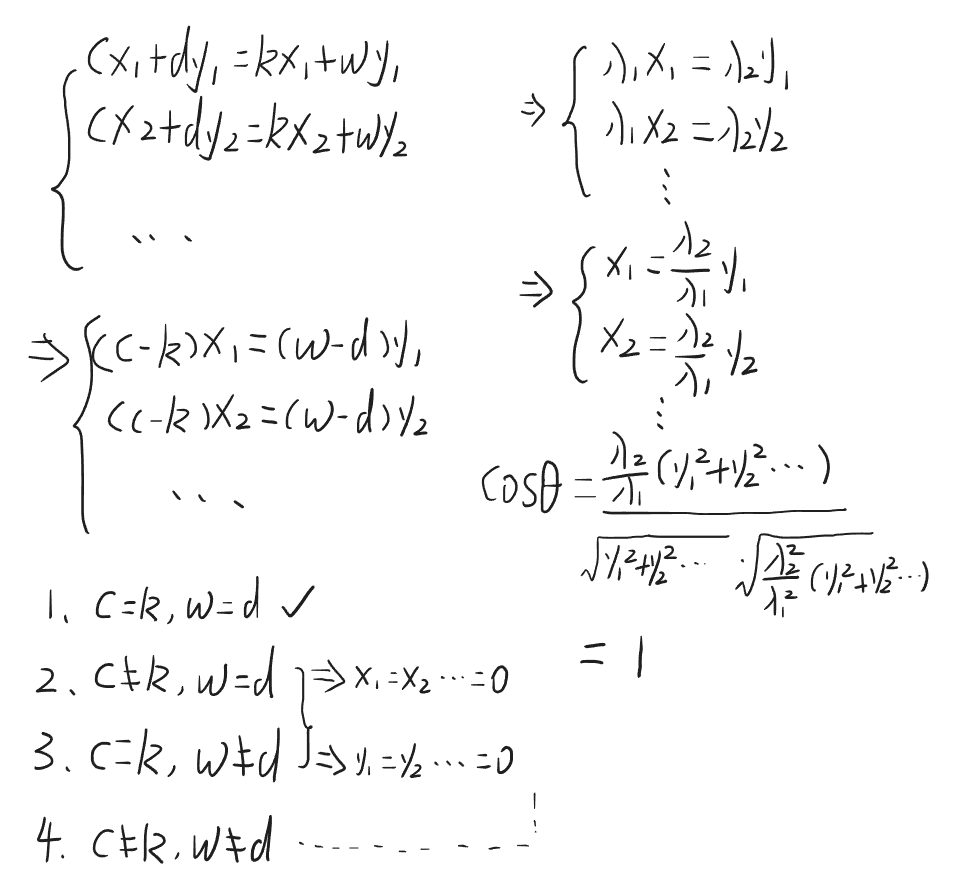
\includegraphics[width=\linewidth ,totalheight=0.95\textheight , keepaspectratio]{线性组合下向量相等的判定.png}
\caption{线性组合下向量相等的判定}
\end{figure}

上面1234四种情况,第一种情况正是我们要证明的,而第二种和第三种情况可以推出某个向量为零向量,这和条件该线性组合可以形成平面冲突。第四种情况可以证明这两个向量的夹角是零,也就是这两个向量是平行的,这也和条件冲突,于是得证。


\subsection{问题集1.1第6题}
\cite{线性代数引论}问题集1.1第6题,作者内心一个潜藏的推理思路是:如果向量的线性组合,可以从中发现某些普遍规律,也就是找到某种关系,使得这个关系不依赖参数c、d...等,那么这个普遍规律对于该线性组合下的所有点都是成立了。【我们太习惯某个事物的局部或者某些特殊情况会更简单一些,常常会忘了在某些时候(这种情况确实很罕见,但也是存在的),该事物从全局从一般情况思考会更简单一些,发现一些普适性的规律,然后自然那些局部的点特殊的情况也一应得到证明了。】

\subsection{问题集1.1第15题}
\cite{线性代数引论}问题集1.1第15题的 $\frac{3}{4}\boldsymbol{v} + \frac{1}{4}\boldsymbol{w}$ 为什么一定在对角线上,证明如下:

\begin{figure}[H]
\centering
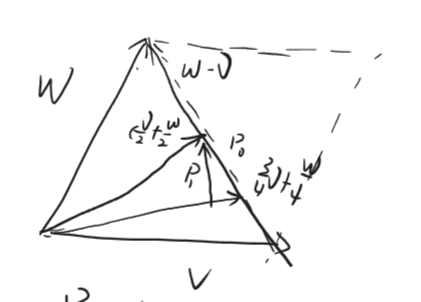
\includegraphics[width=\linewidth ,totalheight=0.95\textheight , keepaspectratio]{线性代数引论问题集1_1_15.png}
\caption{线性代数引论问题集1.1.15}
\end{figure}

已知该对角线为 $\boldsymbol{w} - \boldsymbol{v}$,标记该向量为 $P_0$,现在假定$\frac{3}{4}\boldsymbol{v} + \frac{1}{4}\boldsymbol{w}$ 射出去之后并没有落在对角线上,从而根据$\frac{1}{2}\boldsymbol{v} + \frac{1}{2}\boldsymbol{w}$ 和$\frac{3}{4}\boldsymbol{v} + \frac{1}{4}\boldsymbol{w}$ 的终点确立向量 $P_1$。【已经证明了$\frac{1}{2}\boldsymbol{v} + \frac{1}{2}\boldsymbol{w}$的终点是落在那条对角线的中点的,这很简单,用简单的三角几何分析即可。】

\begin{align*}
P_1 &= \frac{v}{2} + \frac{w}{2} - (\frac{3v}{4} + \frac{w}{4}) \\
    &= -\frac{1}{4}v + \frac{w}{4} \\
    &= \frac{1}{4}(w-v) \\    
 => P_1 // P_0
\end{align*}

因为 $\frac{1}{2}\boldsymbol{v} + \frac{1}{2}\boldsymbol{w}$ 在那条对角线的上,所以 $\frac{3}{4}\boldsymbol{v} + \frac{1}{4}\boldsymbol{w}$ 一定在这条对角线上。上面的证明过程还证明了 $P_1$ 的长度是1/4对角线长度,其终点位置刚好是对角线下面1/4的位置。

上面的证明还可以继续推广,问向量$\boldsymbol{v}$和向量$\boldsymbol{w}$组成的线性组合$c\boldsymbol{v} + d\boldsymbol{w}$ ,$c$和$d$满足何种约束条件就能让其都落在中间那条对角线也就是 $\boldsymbol{w} - \boldsymbol{v}$ 上。

证明如下,其中用到了上面提及的线性组合下向量相等的判定:

\begin{figure}[H]
\centering
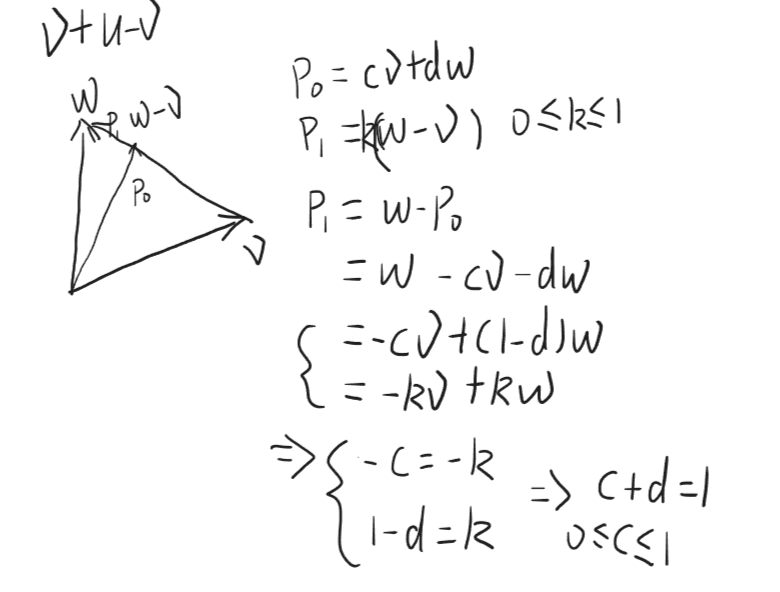
\includegraphics[width=\linewidth ,totalheight=0.95\textheight , keepaspectratio]{线性代数引论问题集1_1_15_2.png}
\end{figure}

最终得证:向量 $P_0 = c\boldsymbol{v}+d\boldsymbol{w}$ ,该向量如果满足 $c+d=1$的条件,则射出去的向量落点会落在中间那条对角线上。


\cite{线性代数引论}问题集1.1第20题将上面讨论的情况扩展到了三个向量的线性组合,问这三个向量的线性组合中,某个向量的系数满足何种条件,该向量的落点在这三个向量终点构成的三角形平面上,有了前面的基础,就很容易得证了。


\begin{figure}[H]
\centering
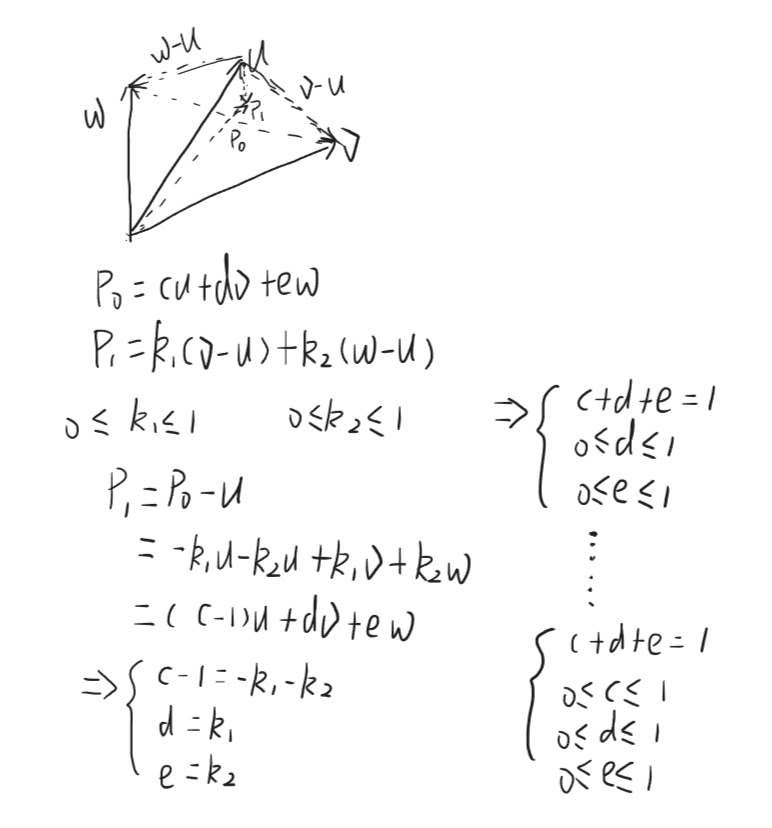
\includegraphics[width=\linewidth ,totalheight=0.95\textheight , keepaspectratio]{线性代数引论问题集1_1_20.png}
\end{figure}


\chapter{术语}
\subsection{当且仅当}
当且仅当的英文是if and only if,常缩写为iff。

A当且仅当B:如果A成立则B成立 ,并且如果A不成立则B不成立【等价于如果B成立则A成立】。

如果命题只有真或者假两种可能性,在所有情况下真值都相同,所以A不成立则B不成立等价于如果B成立则A成立。

\begin{table}[H]
\begin{tabular}{@{}llllll@{}}
\toprule
{A} & {B} & {¬A} & {¬B} & {¬A→¬B} & {B→A} \\ \midrule

{T}          & {T} & {F}  & {F}  & {T}     & {T}   \\
\rowcolor[HTML]{FFFFFF} 
{T}          & {F} & {F}  & {T}  & {T}     & {T}   \\
\rowcolor[HTML]{FFFFFF} 
{F}          & {T} & {T}  & {F}  & {F}     & {F}   \\
\rowcolor[HTML]{FFFFFF} 
{F}          & {F} & {T}  & {T}  & {T}     & {T}   \\ \bottomrule
\end{tabular}
\end{table}


\chapter{约定}
向量一般默认为列向量。可以写为 $(x_1, x_2...)$ 或者 :

\[
\begin{bmatrix}x_{1}  \\ x_2 \\ \vdots \end{bmatrix}
\]

行向量则写为 $[x_1, x_2...]$


\part{附录:编程知识}
编程知识介绍以markdown或者ipynb notebook的形式散落各处,而且只关注介绍28法则中那些最常用最核心的知识点,集中学习一段时间即可,后续应用中若用疑问可搜索可问AI或者查看官方文档等。


\chapter{python语言核心教程}
\href{https://a358003542.github.io/articles/python-core-tutorial.html}{python语言核心教程}



\chapter{numpy基础}
\href{https://github.com/a358003542/ipynb_notebook/blob/master/linear_algebra/numpy_basic.ipynb}{numpy basic}


\chapter{pandas基础}
\href{https://github.com/a358003542/ipynb_notebook/blob/master/linear_algebra/pandas_basic.ipynb}{pandas basic}

\chapter{matplotlib基础}
\href{https://github.com/a358003542/ipynb_notebook/blob/master/matplotlib_basic.ipynb}{matplotlib basic}

\chapter{pytorch基础}
\href{https://github.com/a358003542/ipynb_notebook/blob/master/neural_network/pytorch_basic.ipynb}{pytorch basic}

\backmatter
\part*{附录:参考资料}
\begin{thebibliography}{99}
\bibitem[线性代数引论]{线性代数引论} 《Introduction to Linear Algebra 5e》 by Gilbert Strang at 2016 .
\bibitem[Dive into Deep Learning](Dive into Deep Learning) 《Dive into Deep Learning》 by Aston Zhang \& Zachary C. Lipton \& Mu Li \& Alexander J. Smola at 2023.
\bibitem[什么是数学](什么是数学) 《什么是数学:对思想和方法的基本研究(第三版)》 by [美] R·柯朗 \& H·罗宾 \&  左平  at 2012.

\end{thebibliography}
\end{document}


